\documentclass[11pt]{article}

\usepackage{verbatim,fullpage,graphicx}
\usepackage{xcolor}
\usepackage[most]{tcolorbox}
\colorlet{verylightgray}{lightgray!70!}
\newtcbox{\enterkey}{on line, 
	boxsep=4pt, left=0pt,right=0pt,top=0pt,bottom=0pt,coltext=blue,
	colframe=white,colback=verylightgray,  
	highlight math style={enhanced},fontupper=\ttfamily
}

\usepackage{tikz}
\graphicspath{{./images/}}
\newcommand{\cd}[1]{\enterkey{#1}}

\begin{document}
	\section{Basic Commands}
\begin{itemize}
	\item \cd{git clone <url>} $\to$ Bring a repository that is hosted somewhere like Github into a folder on your local machine
	
	\item \cd{git add <file>} $\to$ Track your files and changes in Git and stage the changes in git
	
	\item \cd{git commit -m "<messege>" <file>} $\to$ Save your files in Git. You can commit like this $$\cd{git commit -m "messege" <file> -m "<description>"}$$ which also gives some description
	
	\item \cd{git push origin <branch-name>} $\to$ Upload Git commits to a remote repo, like Github
	
	\item \cd{git pull} $\to$ Download changes from remote repo to your local machine, the opposite of push
	\item \cd{git status} $\to$ Shows all the files that are created and commited and haven't been commited
\end{itemize}
\section{Initialize a Repo}
\begin{itemize}
	\item Create a folder let \cd{repo}
	\item Create a \cd{README.md} file 
	\item Run the command \cd{git init}
	\item Then add the file by \begin{align*}
		&\cd{git add README.md}\\
		&\cd{git commit -m "Created readme"}
	\end{align*}
	The command \cd{git commit -am "<messege>"} adds and commits but it only works for modified files not newly created files
	\item Now we can not just \cd{git push origin master} since git does not know where to push this since there is no connection. We have to create this connection
	\item Go to github and create an empty repository. Copy the given link
	\item Then run \cd{git remote add origin <copied-url>}
	\item Then run \cd{git push origin master}
	\item Later we will use only \cd{git push} but we will use something called upstream meaning this is where i want to push by default by \cd{git push -u origin master}
\end{itemize}
\begin{figure}[h]
	\centering
	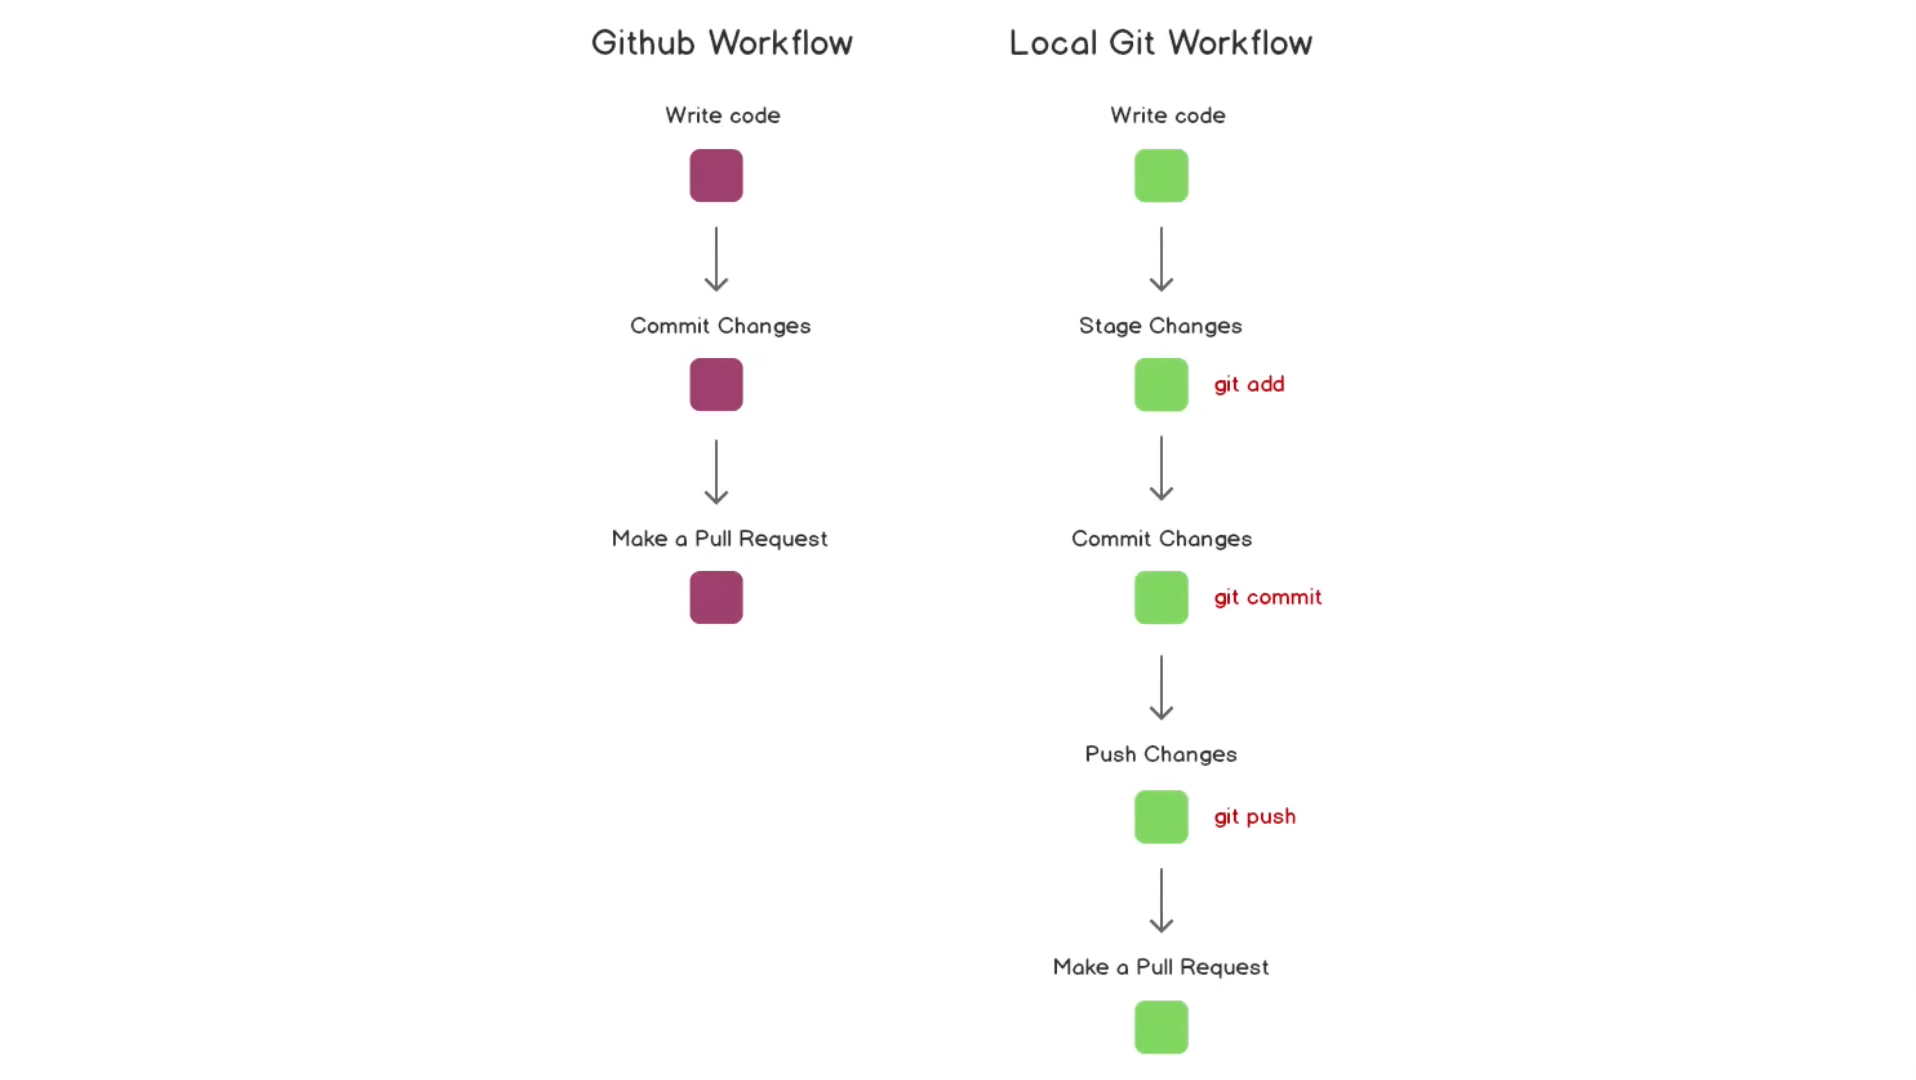
\includegraphics[width=14cm]{git-workflow.png}
\end{figure}

\section{Git Branching} 
By defautl it is the \textit{Master} branch now \textit{Main} branch. We can also create other branches. The more branches you have it more an more looks like a tree. 

\begin{itemize}
	\item Suppose we create another branch \textit{Feature Branch}
	\item At first the code on both branches will be exactly same. 
	\item As you make changes in \textit{Feature Branch} those changes are only visible in \textit{Feature Branch}. Not visible if you swith to \textit{Master Branch}. Same for \textit{Master Branch} changes
	\item Then if you want you can merge it back to Master branch
\end{itemize}
\begin{figure}[h]
	\centering
	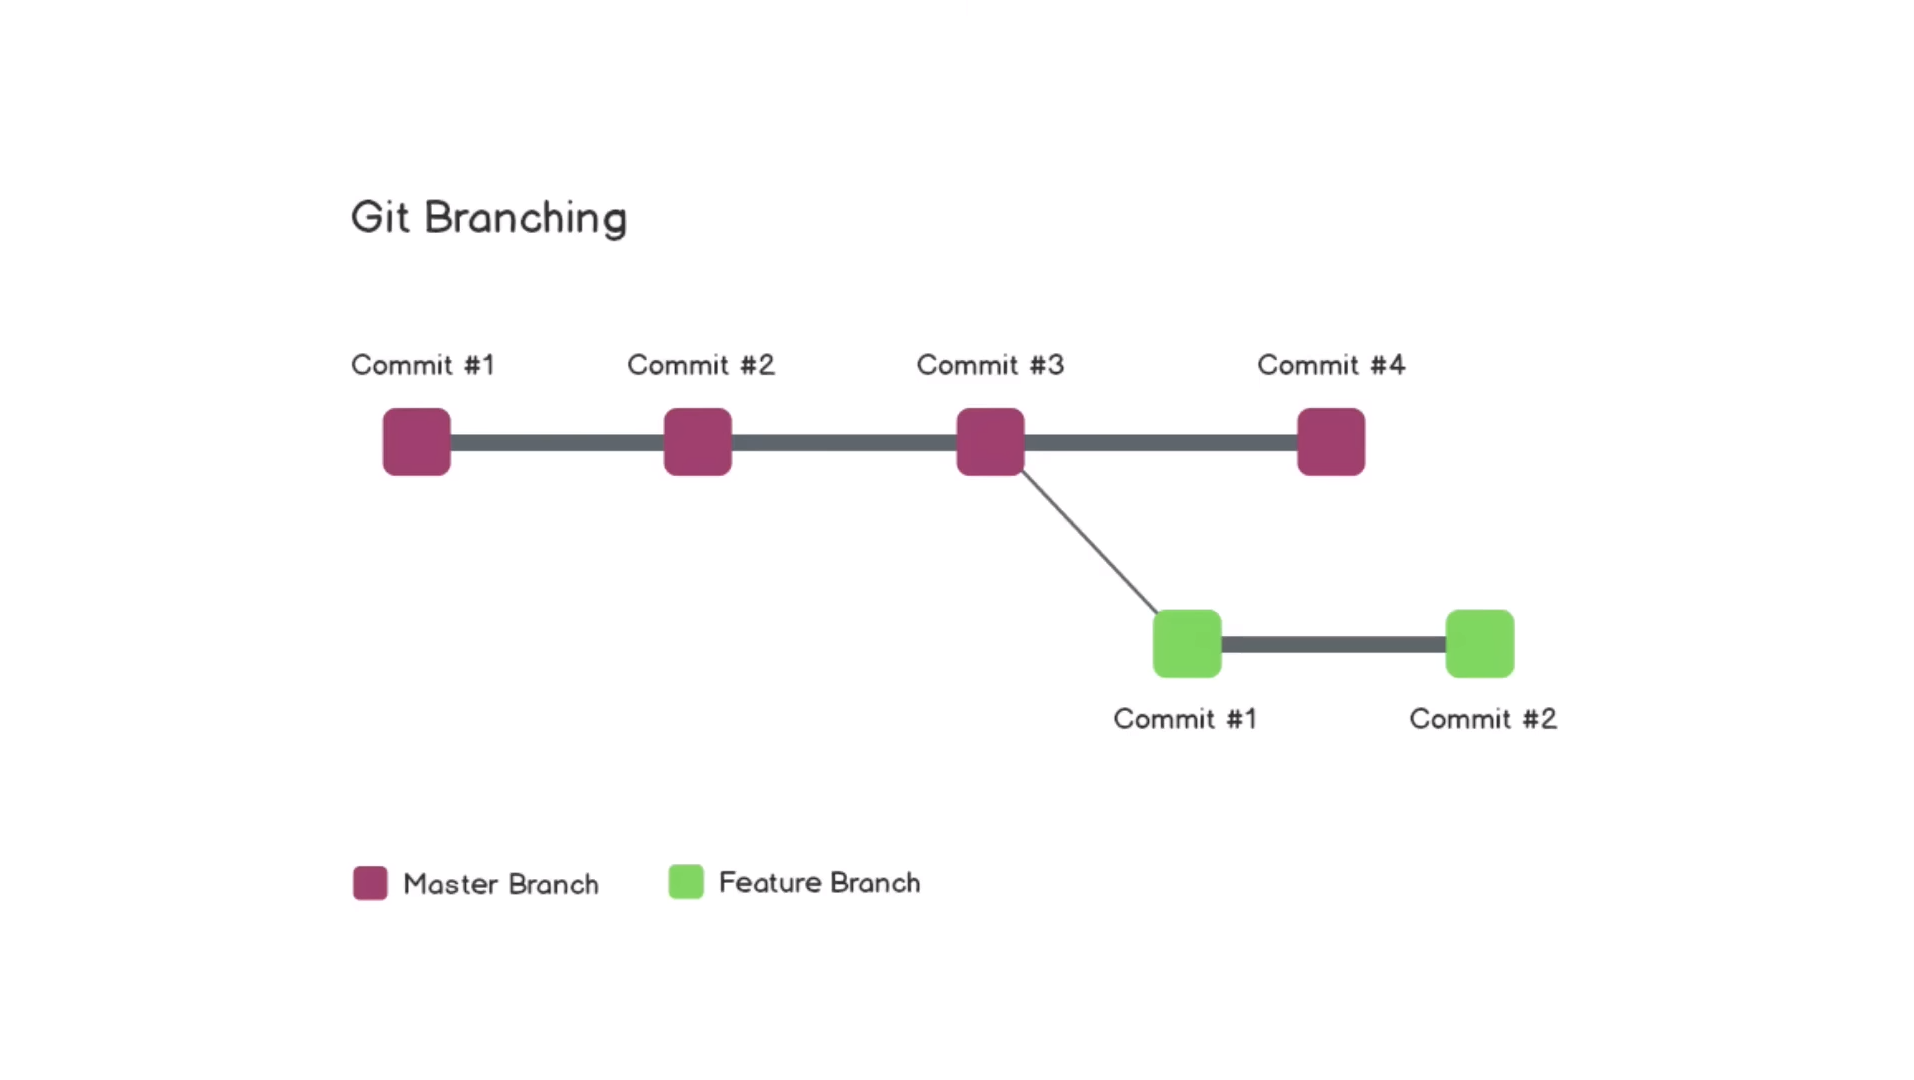
\includegraphics[width=12cm]{branches.png}
\end{figure}
\begin{itemize}
	\item If you run \cd{git branch} it shows  and the branch we are currently in is marked by a *
	\item With \cd{git checkout} you switch between branches. Withour commiting the changes or stash you can not change branch otherwise the changes will be overwritten
	\item To create new branch you run $$\cd{git checkout -b <branch-name>}$$ and it then switches to that newly created branches
	\item \cd{git diff} shows all the changes that havent been committed since last commit. But \cd{git diff <branch>} shows all the difference between current branch and the specified branch
	\item Now you can merge the specified branch with the current branch by \cd{git merge <branch>}
	\item But more common practice is pushing the changes upto github and make a \textit{Pull Request}
	\item While pushing if we are on a different branch in the git push command the branch name will be changed.
\end{itemize}

For \cd{git merge} if you are on branch \textit{A} and you have another branch \textit{B} then \cd{git branch B} makes the merge direction $A\leftarrow B$
\section{Pull Request (PR)}
\begin{itemize}
	\item So will make a PR from the Feature branch to Master branch. 
	\item Once you do a PR ayone can comment on that PR. 
	\item After making a PR you can also update the code and making commits and pushing to the github as long as its on the same branch that you are making th PR with.
	\item Once the PR is merged you generally delete the Feature branch and switch back to the master branch and if you want to make additional coding changes then create new branch adn start the process again
	\item You can merge the PR in github page 
	\item Now locally we dont have the changes.
	\item We need to pull them down to local. To get the changes in our local Master branch from origin we will do \cd{git pull origin master}
	\item We can always remove the branch name from \cd{git pull origin master} by setting the upstream
	\item We still have the branch even after the PR merge. So we will delete the Feature Branch by \cd{git branch -d <branch>}
\end{itemize}


You can also comment on a specific line change in a PR by hittiing the `$+$' button
\begin{figure}[h]
	\centering
	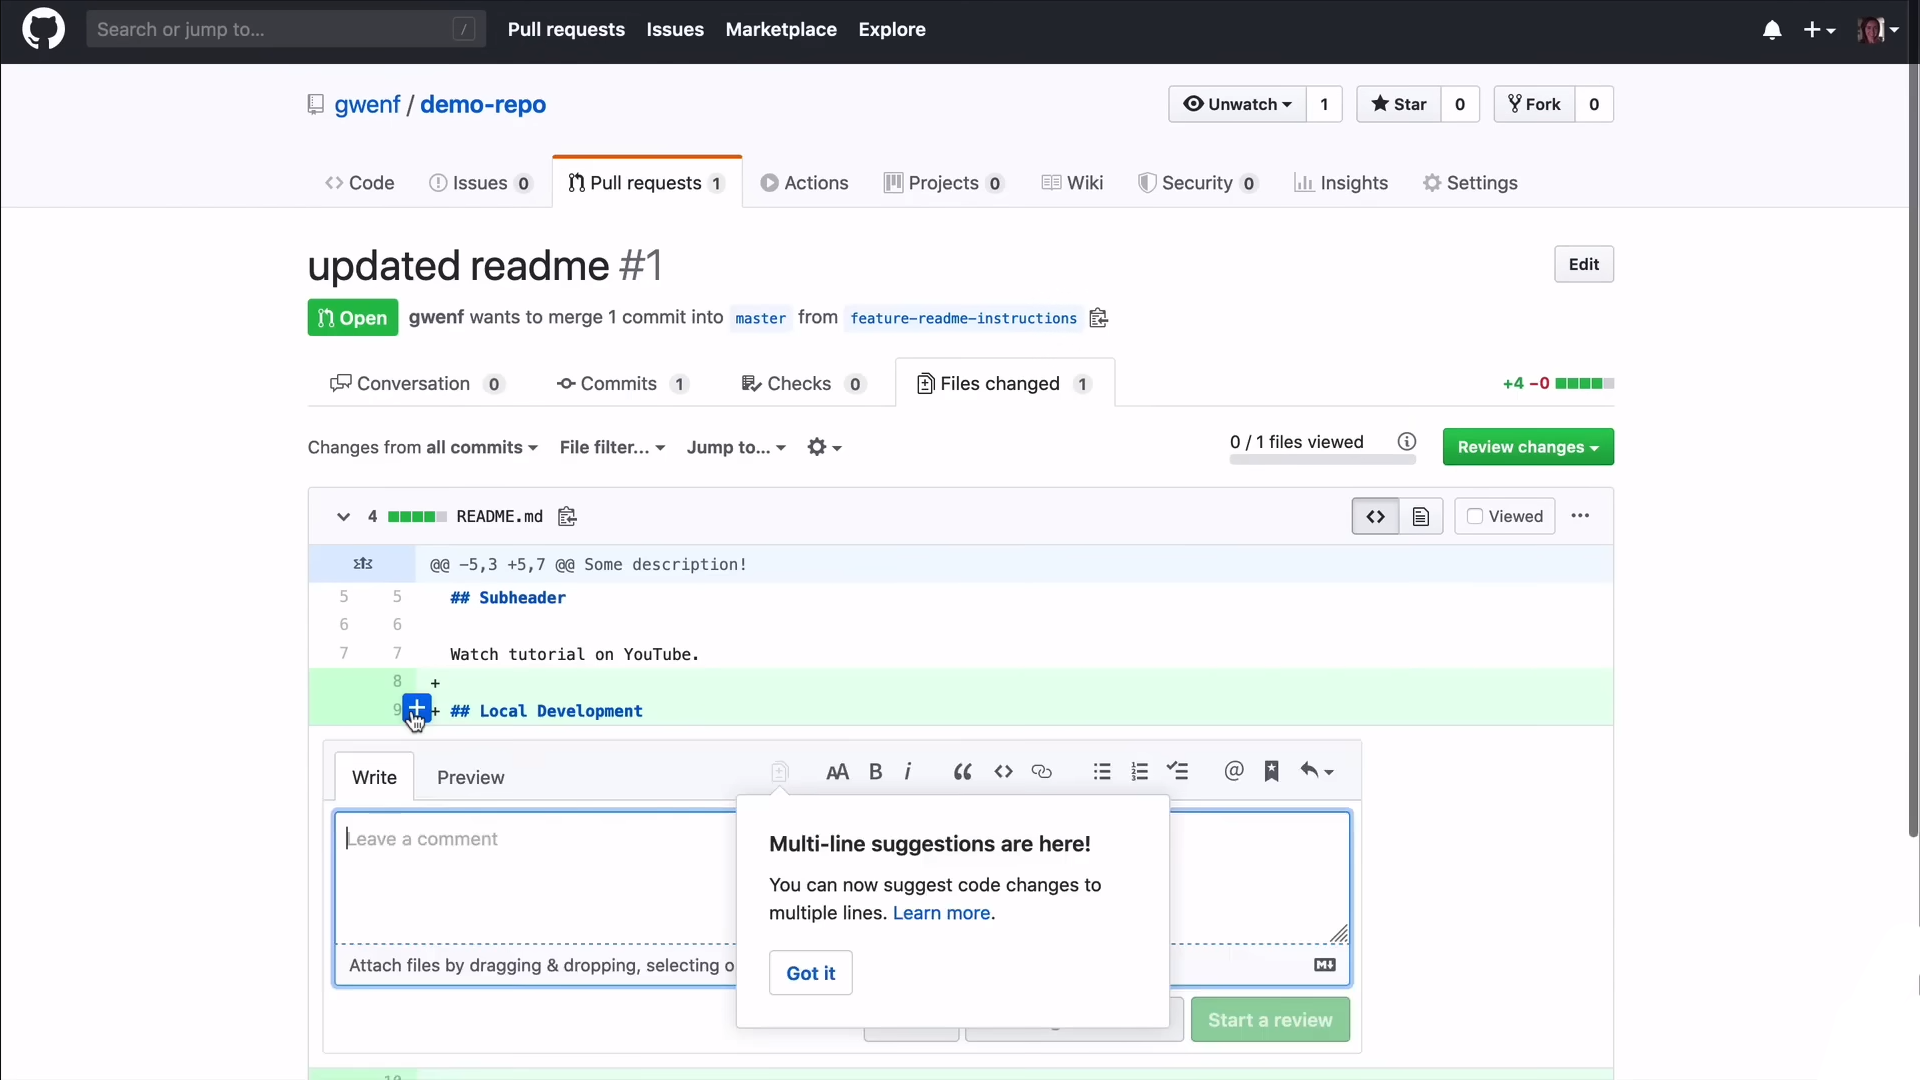
\includegraphics[width=12cm]{comment-on-pr.png}
\end{figure}
In real life it is not easy merging. There is something called \textbf{Merge Conflict}. You building your own code on your own branch. Other people are writing their own code in their own branches. And master is getting updated from multiple different places. SO its possible for multiple people to change the same file. So git doesn't know which code is to keep which code is redundant which code you want to get rid of. You have to manually do that.

To fix merge conflict github gives an interface to fix them. Also you can change with terminal. Then you have to commit the changes then \cd{git merge}.

\section{Undoing}
\begin{itemize}
	\item After staging a file if you want to undo then do \cd{git reset [<file-name>]} Then the file is no longer staged
	\item After commiting if you want to undo the commit do $$\cd{git reset HEAD$\sim$1}$$Here the \cd{HEAD} is a pointer to the last commit. So i am telling it to do something with the last commit. Then \cd{$\sim$1} tells git to instead of pointing to the last commit go one commit further that will completely undo the last commit
	\item Instead of last commit if you want to go some specific commit you can get the hash of that commit from \cd{git log} and then use instad of \cd{HEAD}. But the changes will be there but not saved in git
	\item To grt rid of all changes from some commit then copy the hash of that commit then do \cd{git reset --hard <commit-hash>}
\end{itemize}

\section{Forking}
Another person's repo you can make a copy for yourself and your updates by \textit{Forking}. After making all your updates you can then do a PR

 
\end{document}


